% This file was converted to LaTeX by Writer2LaTeX ver. 1.6.1
% see http://writer2latex.sourceforge.net for more info
\documentclass[twoside]{article}
\usepackage[utf8]{inputenc}
\usepackage{amsmath}
\usepackage{amssymb,amsfonts,textcomp}
\usepackage[T2A,LGR,T1]{fontenc}
\usepackage[greek,russian]{babel}
\usepackage{color}
\usepackage[paperwidth=6.6902in,paperheight=9.45in,top=0.8799in,bottom=0.75in,left=0.9in,right=0.75in,nohead,nofoot]{geometry}
\usepackage{array}
\usepackage{hhline}
\usepackage{hyperref}
\hypersetup{pdftex, colorlinks=true, linkcolor=blue, citecolor=blue, filecolor=blue, urlcolor=blue, pdftitle=}
\usepackage[pdftex]{graphicx}
% Text styles
\newcommand\textstylexixiiipt[1]{\textmd{\textup{\textcolor{black}{#1}}}}
\newcommand\textstylex[1]{\textbf{\textup{#1}}}
\newcommand\textstyleSubtleEmphasis[1]{\textmd{\textit{\textcolor[rgb]{0.0,0.0,0.039215688}{#1}}}}
\newcommand\textstyleEndnodeLink[1]{\textmd{\textcolor[rgb]{0.0,0.0,0.039215688}{#1}}}
\newcommand\textstyleHeadiFirstLine[1]{\textbf{\textup{\MakeUppercase{#1}}}}
\newcommand\textstyleHeadiiFirstLine[1]{\textbf{\textsc{#1}}}
\newcommand\textstyleHeadiiiFirstLine[1]{\textmd{\textit{\MakeUppercase{#1}}}}
\newcommand\textstylexxxiiiviiivpt[1]{\textbf{\textit{\textcolor{black}{#1}}}}
\newcommand\textstyleHeadviiFirstLine[1]{#1}
\newcommand\textstylexxxviii[1]{\textmd{\textup{#1}}}
% Footnote rule
\setlength{\skip\footins}{0.0469in}
\renewcommand\footnoterule{\vspace*{-0.0071in}\setlength\leftskip{0pt}\setlength\rightskip{0pt plus 1fil}\noindent\textcolor{black}{\rule{0.0\columnwidth}{0.0071in}}\vspace*{0.0398in}}
\title{}
\begin{document}
\clearpage\setcounter{page}{1}{\centering
\textsuperscript{ГЕГЕЛЬ}
\par}

{\centering
\textstylexixiiipt{НАУКА ЛОГИКИ}
\par}

{\centering
\textstylexixiiipt{т.~I. Объективная логика}
\par}


\bigskip

{\centering
\textit{перевод}
\par}

{\centering
\textit{Б. Г. СТОЛПНЕРА}
\par}


\bigskip

{\centering
\textit{под редакцией}
\par}

{\centering
\textit{М. Б. МИТИНА}
\par}


\bigskip

\clearpage\setcounter{page}{1}{\itshape
\textup{УДК 14}}

{\itshape
\textup{ББК Ю4,0{\textquotedbl}XIX{\textquotedbl}}}

{\itshape
\textup{Г27}}

\textbf{Гегель.}

Г27\ \ \ \ \textbf{Наука логики. Том I. Объективная логика} [пер. с нем.
Б.~Г.~Столпнера]. — Primedia E-launch LLC, 2017 —
\pageref{bkm:bmEndContent}~с.

\textbf{ISBN 978-1-64008-540-4}

«Наука логики» —~важнейшее сочинение Гегеля, где рельефно выступает его
диалектический метод. Классики марксизма- ленинизма высоко ценят этот труд
Гегеля.

Ленин писал, что «нельзя вполне понять «Капитала» Маркса и особенно его I
главы, не проштудировав и не поняв всей Логики Гегеля». Гегель угадал
диалектику вещей в диалектике понятий. Диалектика Гегеля идеалистична,
поэтому Ленин писал: «Логику Гегеля нельзя применять в данном ее виде;
нельзя брать как данное. Из нее надо выбрать логические (гносеологические)
оттенки, очистив от мистики идей: это еще большая работа».

«Наука логики» Гегеля дается в новом переводе.

{\itshape
\textbf{\textup{ISBN 978-1-64008-540-4}}\textup{\ \ УДК 14}}

{\itshape
\textup{\ \ ББК Ю4,0{\textquotedbl}XIX{\textquotedbl}}}


\bigskip

Главный редактор \textit{М.\hspace{0.25em}В.\hspace{0.25em}Попов}

Корректоры \textit{Н.\hspace{0.25em}А.\hspace{0.25em}Гуринович,
А.\hspace{0.25em}В.\hspace{0.25em}Кузьмин,
В.\hspace{0.25em}А.\hspace{0.25em}Ломов}

Художественное оформление
\textit{Н.\hspace{0.25em}А.\hspace{0.25em}Гуринович,
В.\hspace{0.25em}А.\hspace{0.25em}Ломов}


\bigskip

Сдано в набор 05.08.2017. Подписано в печать 27.07.2017. \newline
Заказ №~2407/17. Формат 70${\times}$100/16. Объём 44,85~усл.~п.~л. 34,5
Уч.-изд.~п.~л.\newline
Бумага офсетная. Тираж 1000 экз. Стоимость за 1 экз.
—~200,00\hspace{0.25em}р.


\bigskip

Издательская фирма «Primedia E-launch LLC»

3900 Swiss Ave, Dallas, TX 75204, USA


\bigskip

Отпечатано в АО «Первая Образцовая типография»

Филиал «Чеховский Печатный Двор»

142300, Московская область, г. Чехов, ул. Полиграфистов, д. 1

Сайт:
\href{http://www.chpk.ru}{\textcolor[rgb]{0.0,0.0,0.039215688}{www}}\href{http://www.chpk.ru}{\textcolor[rgb]{0.0,0.0,0.039215688}{.}}\href{http://www.chpk.ru}{\textcolor[rgb]{0.0,0.0,0.039215688}{chpk}}\href{http://www.chpk.ru}{\textcolor[rgb]{0.0,0.0,0.039215688}{.}}\href{http://www.chpk.ru}{\textcolor[rgb]{0.0,0.0,0.039215688}{ru}}.
E-mail:
\href{mailto:marketing@chpk.ru}{\textcolor[rgb]{0.0,0.0,0.039215688}{marketing@chpk.ru}}

факс 8 (496) 726-54-10, тел. 8 (495) 988-63-87


\bigskip

{\itshape
\textup{Книга напечатана при поддержке Фонда Рабочей Академии
(}\href{http://rpw-mos.ru/}{\textup{rpw-mos.ru}}\textup{), финансовая
поддержка В.\hspace{0.25em}А.\hspace{0.25em}Ломова.}}


\bigskip

\clearpage\setcounter{page}{1}
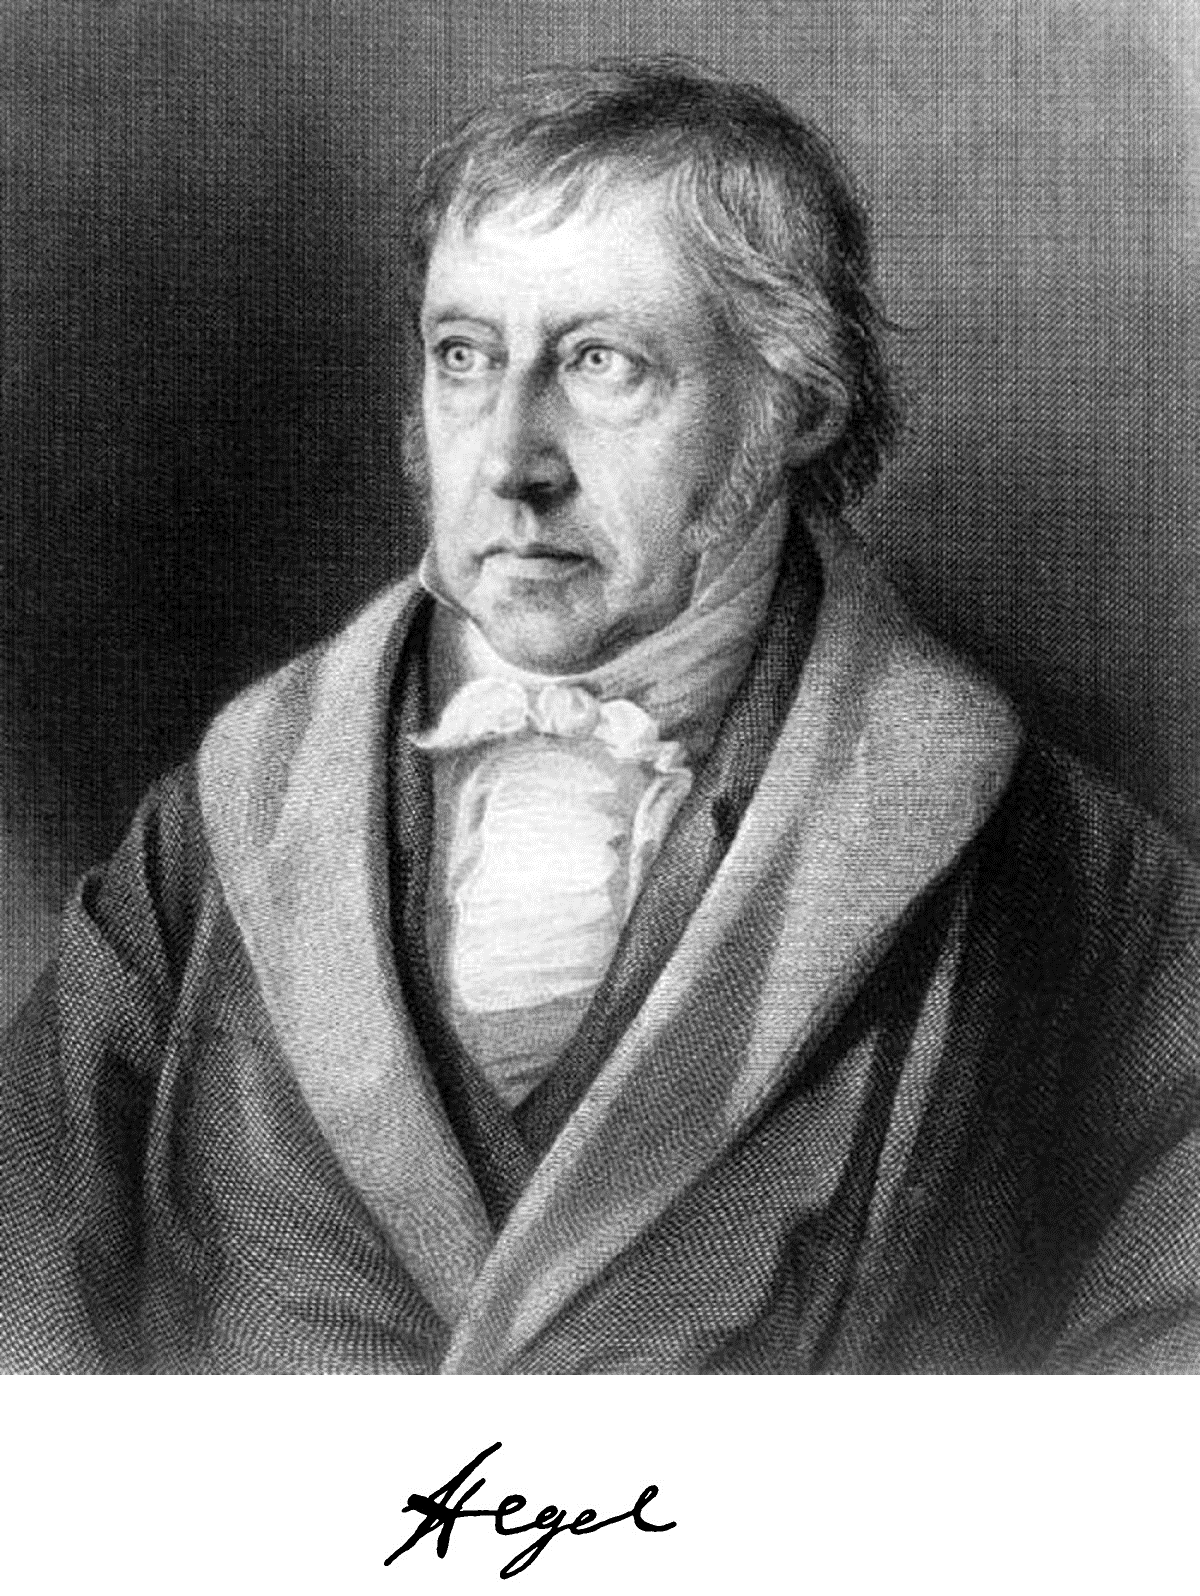
\includegraphics[width=4.0937in,height=5.4457in]{hegel-img001.png} 


\bigskip

\clearpage\setcounter{page}{4}\subsubsection{О значении воинствующего
материализма.}
\label{bkm:Ref474526580}\hypertarget{Toc478978576}{}Об общих задачах
журнала: «Под знаменем марксизма» тов. Троцкий в №~1–2
сказал уже все существенное и сказал прекрасно. Мне хотелось бы
остановиться на некоторых вопросах, ближе определяющих содержание и
программу той работы, которая провозглашена редакцией журнала во
вступительном заявлении к №~1–2.

В этом заявлении говорится, что не все объединившиеся вокруг журнала: «Под
знаменем марксизма» —~коммунисты, но все последовательные материалисты. Я
думаю, что этот союз коммунистов с некоммунистами является безусловно
необходимым и правильно определяет задачи журнала. Одной из самых больших и
опасных ошибок коммунистов (как и вообще революционеров, успешно
проделавших начало великой революции) является представление, будто бы
революцию можно совершить руками одних революционеров. Напротив, для успеха
всякой серьезной революционной работы необходимо понять и суметь претворить
в жизнь, что революционеры способны сыграть роль лишь как авангард
действительно жизнеспособного и передового класса. Авангард лишь тогда
выполняет задачи авангарда, когда он умеет не отрываться от руководимой им
массы, а действительно вести вперед всю массу. Без союза с некоммунистами в
самых различных областях деятельности ни о каком успешном коммунистическом
строительстве не может быть и речи.

Это относится и к той работе защиты материализма и марксизма, за которую
взялся журнал: «Под знаменем марксизма». У главных направлений передовой
общественной мысли России имеется, к счастью, солидная материалистическая
традиция. Не говоря уже о
Г.\textlatin{[202F?]}В.\textlatin{[202F?]}Плеханове, достаточно назвать
Чернышевского, от которого современные народники (народные социалисты,
с.-р. и~т.~п.) отступали назад нередко в погоне за модными реакционными
философскими учениями, поддаваясь мишуре якобы «последнего слова»
европейской науки и не умея разобрать под этой мишурой той или иной
разновидности прислужничества буржуазии, ее предразсудкам и буржуазной
реакционности.

Во всяком случае, у нас в России есть еще и довольно долго, несомненно,
будут материалисты из лагеря некоммунистов, и наш безусловный долг
привлекать к совместной работе всех сторонников последовательного и
воинствующего материализма в борьбе с философской реакцией и с философскими
предразсудками так называемого «образованного общества». Дицген-отец,
которого не надо смешивать с его, столь же претенциозным, сколь неудачным
литератором-сынком, выразил правильно, метко и ясно основную точку зрения
марксизма на господствующие в буржуазных странах и пользующиеся среди их
ученых и публицистов вниманием философские направления, сказавши, что
профессора философии в современном обществе представляют из себя в
большинстве случаев на деле ни что иное, как «дипломированных лакеев
поповщины».

Наши российские интеллигенты, любящие считать себя передовыми, как, впрочем,
и их собратия во всех остальных странах, очень не любят перенесения вопроса
в плоскость той оценки, которая дана словами Дицгена. Но не любят они этого
потому, что правда колет глаза. Достаточно сколько-нибудь вдуматься в
государственную, затем общеэкономическую, затем бытовую и всяческую иную
зависимость современных образованных людей от господствующей буржуазии,
чтобы понять абсолютную правильность резкой характеристики Дицгена.
Достаточно вспомнить громадное большинство модных философских направлений,
которые так часто возникают в европейских странах, начиная, хотя бы, с тех,
которые были связаны с открытием радия, и кончая теми, которые теперь
стремятся уцепиться за Эйнштейна, — чтобы представить себе связь между
классовыми интересами н классовой позицией буржуазии, поддержкой ею
всяческих форм религий и идейным содержанием модных философских
направлений.

Из указанного видно, что журнал, который хочет быть органом воинствующего
материализма, должен быть боевым органом во-первых, в смысле неуклонного
разоблачения и преследования всех современных «дипломированных лакеев
поповщины», все равно, выступают ли они в качестве представителей
официальной науки или в качество вольных стрелков, называющих себя
«демократическими левыми или идейно социалистическими публицистами».

Такой журнал должен быть, во-вторых, органом воинствующего атеизма. У нас
есть ведомства или, по крайней мере, государственные учреждения, которые
этой работой ведают. Но ведется эта работа крайне вяло, крайне
неудовлетворительно, испытывая, видимо, на себе гнет общих условий нашего
истинно русского (хотя и советского) бюрократизма. Чрезвычайно существенно
потому, чтобы в дополнение к работе соответствующих государственных
учреждений, в исправление ее и в оживление ее, журнал, посвящающий себя
задаче стать органом воинствующего материализма, вел неутомимую
атеистическую пропаганду и борьбу. Надо внимательно следить за всей
соответствующей литературой на всех языках, переводя или, по крайней мере,
реферируя все сколько-нибудь ценное в этой области.

Энгельс давно советовал руководителям современного пролетариата переводить
для массового распространения в народе боевую атеистическую литературу
конца 18 века. К стыду нашему, мы до сих пор этого по сделали (одно из
многочисленных доказательств того, что завоевать власть в революционную
эпоху гораздо легче, чем суметь правильно этою властью пользоваться).
Иногда оправдывают эту нашу вялость, бездеятельность и неумелость
всяческими «выспренними» соображениями: например, «дескать, старая
атеистическая литература 18-го века устарела, ненаучна, наивна» и~т.~п. Нет
ничего хуже подобных, якобы ученых, софизмов, прикрывающих либо педантство,
либо полное непонимание марксизма. Конечно, и ненаучного, и наивного
найдется не мало в атеистических произведениях революционеров 18-го века.
Но никто не мешает издателям этих сочинений сократить их и снабдить
короткими послесловиями с указанием на прогресс научной критики религий,
проделанный человечеством с конца 18-го века, с указанием на
соответствующие новейшие сочинения и~т.~д. Было бы величайшей ошибкой и
худшей ошибкой, которую может сделать марксист, думать, что многомиллионные
народные (особенно, крестьянские и ремесленные) массы, осужденные всем
современным обществом за темноту, невежество и предрассудки, могут
выбраться из этой темноты только по прямой линии чисто марксистского
просвещения. Этим массам необходимо дать самый разнообразный материал по
атеистической пропаганде, знакомить их с фактами из самых различных
областей жизни, подойти к ним и так и этак для того, чтобы их
заинтересовать, пробудить их от религиозного сна, встряхнуть их с самых
различных сторон, самыми различными способами и~т.~п.

Бойкая, живая, талантливая, остроумно и открыто нападающая на господствующую
поповщину публицистика старых атеистов 18-го века сплошь н рядом окажется в
1000 раз более подходящей для того, чтобы пробудить людей от религиозного
сна, чем скучные, сухие, не иллюстрированные почти никакими умело
подобранными фактами, пересказы марксизма, которые преобладают в нашей
литературе и которые (нечего греха таить) часто марксизм искажают. Все
сколько-нибудь крупные произведения Маркса и Энгельса у нас переведены.
Опасаться, что старый атеизм и старый материализм останутся у нас
недополненными теми исправлениями, которые внесли Маркс и Энгельс, нет
решительно никаких оснований. Самое важное—чаще всего именно это забывают
наши якобы марксистские, а на самом деле уродующие марксизм коммунисты
—~это суметь заинтересовать совсем еще неразвитые массы сознательным
отношением к религиозным вопросам и сознательной критикой религий.

С другой стороны, взгляните на представителей современной научной критики
религий. Почти всегда эти представители образованной буржуазии «дополняют»
свое же собственное опровержение религиозных предрассудков такими
рассуждениями, которые сразу разоблачают их как идейных рабов буржуазии,
как «дипломированных лакеев поповщины».

Два примера. Проф. Р.\textlatin{[202F?]}Ю.\textlatin{[202F?]}Виппер издал в
1918 году книжечку: «Возникновение христианства» (изд. «Фарос». Москва).
Пересказывая главные результаты современной науки, автор не только не воюет
с предрассудками и с обманом, которые составляют оружие церкви, как
политической организации, не только обходит эти вопросы, но заявляет прямо
смешную и реакционнейшую претензию подняться выше обеих «крайностей»: и
идеалистической и материалистической. Это —~прислужничество господствующей
буржуазии, которая во всем мире сотни миллионов рублей из выжимаемой ею с
трудящихся прибыли употребляет на поддержку религии.

Известный немецкий ученый, Артур Древс, опровергая в своей книге: «Миф о
Христе» религиозные предрассудки и сказки, доказывая, что никакого Христа
не было, в конце книги высказывается за религию, только подновленную,
подчищенную, ухищренную, способную противостоять «ежедневно все более и
более усиливающемуся натуралистическому потоку» (стр.~238, 4-го немецкого
издания, 1910 года). Это —~реакционер прямой, сознательный, открыто
помогающий эксплуататорам заменять старые и прогнившие религиозные
предрассудки новенькими, еще более гаденькими и подлыми предрассудками.

Это не значит, чтобы не надо было переводить Древса. Это значит, что
коммунисты и все последовательные материалисты должны, осуществляя в
известной мере свой союз с прогрессивной частью буржуазии, неуклонно
разоблачать ее, когда она впадает в реакционность. Это значит, что чураться
союза с представителями буржуазии 18-го века,~т.~е. той эпохи, когда она
была революционной, значило бы изменять марксизму и материализму, ибо
«союз» с Древсами в той или иной форме, в той или иной степени, для нас
обязателен в борьбе с господствующими религиозными мракобесами.

Журнал: «Под знаменем марксизма», который хочет быть органом воинствующего
материализма, должен уделять много места атеистической пропаганде, обзору
соответствующей литературы и исправлению громадных недочетов пашей
государственной работы в этой области. Особенно важно использование тех
книг и брошюр, которые содержат много конкретных фактов и сопоставлений,
показывающих связь классовых интересов и классовых организаций современной
буржуазии с организациями религиозных учреждений и религиозной пропаганды.

Чрезвычайно важны все материалы, относящиеся к Соединенным Штатам Северной
Америки, в которой меньше проявляется официальная, казенная,
государственная связь религии и капитала. Но зато нам яснее становится, что
так называемая «современная демократия» (перед которой так неразумно
разбивают свой лоб меньшевики, с.-р. и отчасти анархисты и~т.~п.)
представляет из себя ни что иное, как свободу проповедывать то, что
буржуазии выгодно проповедывать, а выгодно ей проповедывать самые
реакционные идеи, религию, мракобесие, защиту эксплуататоров и~т.~п.

Хотелось бы надеяться, что журнал, который хочет быть органом воинствующего
материализма, даст нашей читающей публике обзоры атеистической литературы с
характеристикой, для какого круга читателей и в каком отношении могли быть
подходящими те или иные произведения и с указанием того, что появилось у
нас (появившимися надо считать только сносные переводы, а их не так много)
и что должно быть еще издано.

Кроме союза с последовательными материалистами, которые не принадлежат к
партии коммунистов, не менее, если не более важен для той работы, которую
воинствующий материализм должен проделать, союз с представителями
современного естествознания, которые склоняются к материализму и не боятся
отстаивать и проповедывать его против господствующих в так называемом
«образованном обществе» модных философских шатаний в сторону идеализма и
скептицизма.

Помещенная в 1–2 номере журнала: «Под знаменем марксизма» статья
А.\textlatin{[202F?]}Тимирязева о теории относительности Эйнштейна
позволяет надеяться, что журналу удастся осуществить и этот второй союз.
Надо обратить на него побольше внимания. Надо помнить, что именно из крутой
ломки, которую переживает современное естествознание, родятся сплошь да
рядом реакционные философские школы и школки, направления и направленьица.
Поэтому следить за вопросами, которые выдвигает новейшая революция в
области естествознания и привлекать к этой работе в философском журнале
естествоиспытателей, — это задача, без решения которой воинствующий
материализм не может быть ни в коем случае ни воинствующим, ни
материализмом. Если Тимирязев в первом номере журнала должен был оговорить,
что за теорию Эйнштейна, который сам, по словам Тимирязева, никакого
активного похода против основ материализма не ведет, ухватилась уже
громадная масса представителей буржуазной интеллигенции всех стран, то это
относится не к одному Эйнштейну, а к целому ряду, если не к большинству
великих преобразователей естествознания, начиная с конца 19-го века.

И для того, чтобы не относиться к подобному явлению бессознательно, мы
должны понять, что без солидного философского обоснования никакие
естественные науки, никакой материализм не может выдержать борьбы против
натиска буржуазных идей и восстановления буржуазного миросозерцания. Чтобы
выдержать эту борьбу и провести ее до конца с полным успехом, естественник
должен быть современным материалистом, сознательным сторонником того
материализма, который представлен Марксом, то-есть должен быть
диалектическим материалистом. Чтобы достигнуть этой цели, сотрудники
журнала «Под знаменем марксизма» должны организовать систематическое
изучение диалектики Гегеля с материалистической точки зрения,~т.~е. той
диалектики, которую Маркс практически применял и в своем «Капитале» и в
своих исторических и политических работах и применял с таким успехом, что
теперь каждый день пробуждения новых классов к жизни и к борьбе на Востоке
(Япония, Индия, Китай) —~т.~е. тех сотен миллионов человечества, которые
составляют большую часть населения земли и которые своей исторической
бездеятельностью и своим исторический сном обусловливали до сих пор застой
и гниение во многих передовых государствах Европы, — каждый день
пробуждения к жизни новых народов и новых классов, все больше и больше
подтверждает марксизм.

Конечно, работа такого изучения, такого истолкования и такой пропаганды
Гегелевской диалектики чрезвычайно трудна, и несомненно, первые опыты в
этом отношении будут связаны с ошибками. Но не ошибается только тот, кто
ничего не делает. Опираясь на то, как применял Маркс материалистически
понятую диалектику Гегеля, мы можем и должны разрабатывать эту диалектику
со всех сторон, печатать в журнале отрывки из главных сочинений Гегеля,
истолковывать их материалистически, комментируя образцами применения
диалектики у Маркса а так же теми образцами диалектики в области отношений
экономических, политических, каковых образцов новейшая история, особенно
современная империалистическая война и революция, дают необыкновенно много.
Группа редакторов и сотрудников журнала: «Под знаменем марксизма» должна
быть на мой взгляд своего рода «обществом материалистических друзей
Гегелевской диалектики.» Современные естествоиспытатели найдут (если сумеют
искать и если мы научимся помогать им) в материалистически истолкованной
диалектике Гегеля ряд ответов на те философские вопросы, которые ставятся
революцией в естествознании и на которых «сбиваются» в реакцию
интеллигентские поклонники буржуазной моды.

Без того, чтобы такую задачу себе поставить и систематически ее выполнять,
материализм не может быть воинствующим материализмом. Он останется,
употребляя щедринское выражение, не столько сражающимся, сколько сражаемым.
Без этого крупные естествоиспытатели так же часто, как и до сих пор, будут
беспомощны в своих философских выводах и обобщениях. Ибо естествознание
прогрессирует так быстро, переживает период такой глубокой революционной
ломки во всех областях, что без философских выводов естествознанию не
обойтись ни в коем случае.

В заключение приведу пример, не относящийся к области философии, но во
всяком случае относящийся к области общественных вопросов, которым также
хочет уделить внимание журнал: «Под знаменем марксизма».

Это один из примеров того, как современная якобы наука на самом деле служит
проводником грубейших и гнуснейших реакционных взглядов.

Недавно мне прислали журнал «Экономист», №\textlatin{[202F?]}1 (1922 г.),
издаваемый XI отделом «Русского технического общества». Приславший мне этот
журнал молодой коммунист (вероятно, не имевший времени ознакомиться с
содержанием журнала) неосторожно отозвался о журнале чрезвычайно
сочувственно. На самом же деле журнал является, не знаю насколько
сознательно, органом современных крепостников, прикрывающихся, конечно,
мантией научности, демократизма и~т.~п.

Некий г.~П.\textlatin{[202F?]}А.\textlatin{[202F?]}Сорокин помещает в этом
журнале обширные, якобы «социологические» исследования «О влиянии войны».
Ученая статья пестрит учеными ссылками на «социологические» труды автора и
его многочисленных заграничных учителей и сотоварищей. Вот какова его
ученость:

На странице 83-й читаю:

«На 10.000 браков в Петрограде теперь приходится 92,2 разводов (цифра
фантастическая), при чем из 100 расторгнутых браков 51,1 были
продолжительностью менее одного года, 11\% менее одного месяца, 22\% менее
двух месяцев, 41 \% менее 3–6-ти месяцев и лишь 26\% свыше 6-ти месяцев.
Эти цифры говорят, что современный легальный брак —~форма, скрывающая по
существу вне-брачные половые отношения и дающая возможность любителям
„клубники“ „законно“ удовлетворять свои аппетиты». («Экономист»
№\textlatin{[202F?]}1, стр. 83-я).

Нет сомнения, что и этот господин, и то русское техническое общество,
которое издает журнал и помещает в нем подобные рассуждения, причисляют
себя к сторонникам демократии и сочтут за величайшее оскорбление, когда их
назовут тем, что они есть на самом деле,~т.~е. крепостниками,
реакционерами, «дипломированными лакеями поповщины».

Самое небольшое знакомство с законодательством буржуазных стран о браке,
разводе и вне-брачных детях, а равно с фактическим положением дела в этом
отношении, покажет любому интересующемуся вопросом человеку, что
современная буржуазная демократия, даже во всех наиболее демократических
буржуазных республиках, проявляет себя в указанном отношении именно
крепостнически по отношению к женщине и по отношению к вне-брачным детям.

Это не мешает, конечно, меньшевикам, с. р. и части анархистов и всем
соответствующим партиям на Западе продолжать кричать о демократии и о ее
нарушении большевиками. На самом деле, именно большевистская революция
является единственной последовательно демократической революцией в
отношении к таким вопросам, как брак, развод и положение вне-брачных детей.
А это вопрос, затрагивающий самим непосредственным образом интересы большей
половины населения в любой стране. Только большевистская революция впервые,
несмотря на громадное число предшествовавших ей и называющих себя
демократическими буржуазных революций, — провела решительную борьбу в
указанном отношении, как против реакционности и крепостничества, так и
против обычного лицемерия правящих и имущих классов.

Если г.\textlatin{[202F?]}Сорокину 92 развода на 10.000 браков кажется
цифрой фантастической, то остается предположить, что либо автор жил и
воспитывался в каком-нибудь, настолько загороженном от жизни монастыре, что
в существование подобного монастыря едва кто-нибудь поверит, либо что этот
автор искажает правду в угоду реакции и буржуазии. Всякий сколько-нибудь
знакомый с общественными условиями в буржуазных странах человек знает, что
фактическое число фактических разводов (конечно, не санкционированных
церковью и законом) повсюду неизмеримо больше. Россия в этом отношении
отличается от других стран только тем, что ее законы не освящают лицемерия
и бесправного положения женщины и ее ребенка, а открыто и от имени
государственной власти объявляют систематическую войну против всякого
лицемерия и всякого бесправия.

Марксистскому журналу придется вести войну и против подобных современных
«образованных» крепостников. Вероятно, немалая их часть получает у нас даже
государственные деньги и состоит на государственной службе для просвещения
юношества, хотя для этой цели они годятся не больше, чем заведомые
растлители годились бы для роли надзирателей в учебных заведениях для
младшего возраста.

Рабочий класс в России сумел завоевать власть, но пользоваться ею еще не
научился, ибо в противном случае, он бы подобных преподавателей и членов
ученых обществ давно бы вежливо препроводил в страны буржуазной
«демократии». Там подобным крепостникам самое настоящее место.

Научится, была бы охота учиться.

{\raggedleft
\textit{Н. Ленин.}
\par}

12 марта 1922 г.


\bigskip
